\documentclass[a4paper, 10pt]{article}
\linespread{1.33}
% ┌─────────────────────┐
% │     preamble.tex    │
% └─────────────────────┘

% ══════════ [1] Basic document settings ══════════
\usepackage{fullpage}
\usepackage{geometry}
\geometry{
    top = 2cm,
    bottom = 4.5cm,
    left = 2.5cm,
    right = 2.5cm
}
\usepackage{lastpage}

\usepackage{xcolor}
\usepackage{graphicx}
\usepackage{tikz}
\usepackage{pgfplots}

\usepackage{enumerate}
\usepackage{sectsty}
\subsectionfont{\color{blue}}
\usepackage{enumitem}
\usepackage{array}
\newcolumntype{P}[1]{>{\centering\arraybackslash}p{#1}}

\usepackage{fourier-orns}
\usetikzlibrary{decorations.text}
\pgfplotsset{compat = newest}
\newcommand{\seprule}{
    \vspace*{1.5em}
    \vspace{-8pt}\hrulefill
    \raisebox{-2.1pt}{\quad\decofourleft\decotwo\decofourright\quad}\hrulefill
    \vspace*{1.5em}
}

\usepackage{hyperref}
\hypersetup{
  colorlinks=true,
  linkcolor=blue,
  linkbordercolor={0 0 1},
  urlcolor=blue
}

\usepackage{fancyhdr}
\usepackage[]{mdframed}

\renewcommand{\thesubsection}{\S{} \arabic{section}.\arabic{subsection}}

% ══════════ [2] Math packages ══════════
\usepackage{amsmath}
\usepackage{amsthm}
\usepackage{amsfonts}
\usepackage{amssymb}
\usepackage{amscd}
\usepackage{mathrsfs}
\usepackage{cancel}

% ══════════ [3] Miscellaneous & Fonts ══════════
\setlength{\parindent}{0.0in}
\setlength{\parskip}{0.05in}
\renewcommand{\footrulewidth}{0.4pt}

\usepackage{mathpazo}
\usepackage{domitian}
\usepackage[T1]{fontenc}
\let\oldstylenums\oldstyle
\setmonofont[Scale = 0.8]{DejaVu Sans Mono}

% ══════════ [4] amsthm setup ══════════

\newtheorem{theorem}{Theorem}[section]
\newtheorem{corollary}[theorem]{Corollary}
\newtheorem{lemma}[theorem]{Lemma}

\theoremstyle{definition}
\newtheorem{definition}[theorem]{Definition}

\theoremstyle{remark}
\newtheorem*{remark}{Remark}

\theoremstyle{definition}
\newtheorem{obs}[theorem]{Observation}

\theoremstyle{definition}
\newtheorem{exercise}[theorem]{Exercise}
\newmdtheoremenv[innertopmargin = 8pt,
                 innerbottommargin = 10pt]{exer}[theorem]{Exercise}

\theoremstyle{definition}
\newtheorem{example}[theorem]{Example}
% ┌─────────────────────┐
% │   usercommand.tex   │
% └─────────────────────┘

% ══════════ [1] short-hand notations ══════════
\newcommand{\mbf}{\mathbf}
\newcommand{\mrm}{\mathrm}
\newcommand{\mca}{\mathcal}
\newcommand{\msc}{\mathsc}
\newcommand{\mbb}{\mathbb}
\newcommand{\msf}{\mathsf}

\newcommand{\tbf}{\textbf}
\newcommand{\tit}{\textit}

\newcommand{\eps}{\epsilon}
\newcommand{\kB}{k_{\mathrm{B}}}
\def\dbar{{\mathchar'26\mkern-12mu d}}
\newcommand{\contradiction}{\ensuremath{{\Rightarrow\mspace{-2mu}\Leftarrow}}}
\newcommand{\im}{\mathrm{im}\,}
\renewcommand{\d}{\mathrm{d}}

\renewcommand\qedsymbol{$\blacksquare$}

\newcommand\lecturenumber{06}
\newcommand\lecturedate{Nov 15, 2024}

\pagestyle{fancyplain}
\headheight 40pt
\lhead{Lecture \lecturenumber\\CNBC Deep Learning Subgroup}
\rhead{Riemannian Geometry for Deep Learning \\\lecturedate}
\cfoot{Fall 2024, SNU}
\rfoot{\small\thepage}
\headsep 1.5em

\begin{document}
\setcounter{section}{4}
\section{Vectors and Tensors on Manifolds}

\subsection{Vectors}

An \tit{elementary} picture of a vector as an arrow connecting a point and the origin does not work in a manifold.
\begin{itemize}
    \item[-] Where is the origin on the manifold?
    \item[-] What is a \tit{straight} arrow on the manifold? For example, how can we define a straight arrow that connects London and Los Angeles on the \tit{surface} or the Earth?
\end{itemize}

Let us look at the \tbf{tangent line} to a curve in $\mbb{R}^{2}$. If the curve is differentiable, the tangent line at $x = x_{0}$ becomes
\[ y - y(x_{0}) = a(x - x_{0}),\quad a = \left.\frac{dy}{dx}\right|_{x_{0}} \]
The tangent vectors on a manifold $\mca{M}$ generalize this tangent line. On a manifold, a vector is defined to be a tangent vector to a \tbf{curve} in $\mca{M}$.

\seprule

\begin{definition}
    Consider a curve $c \,:\, (a,b) \rightarrow \mca{M}$ and a smooth function $f \,:\, \mca{M} \rightarrow \mbb{R}$. The \tbf{tangent vector} at $c(0)$ is defined as a \tbf{directional derivative} of a function $f(c(t))$ along the curve $c(t)$ at $t = 0$.

    \begin{figure}[htbp]
        \centering
        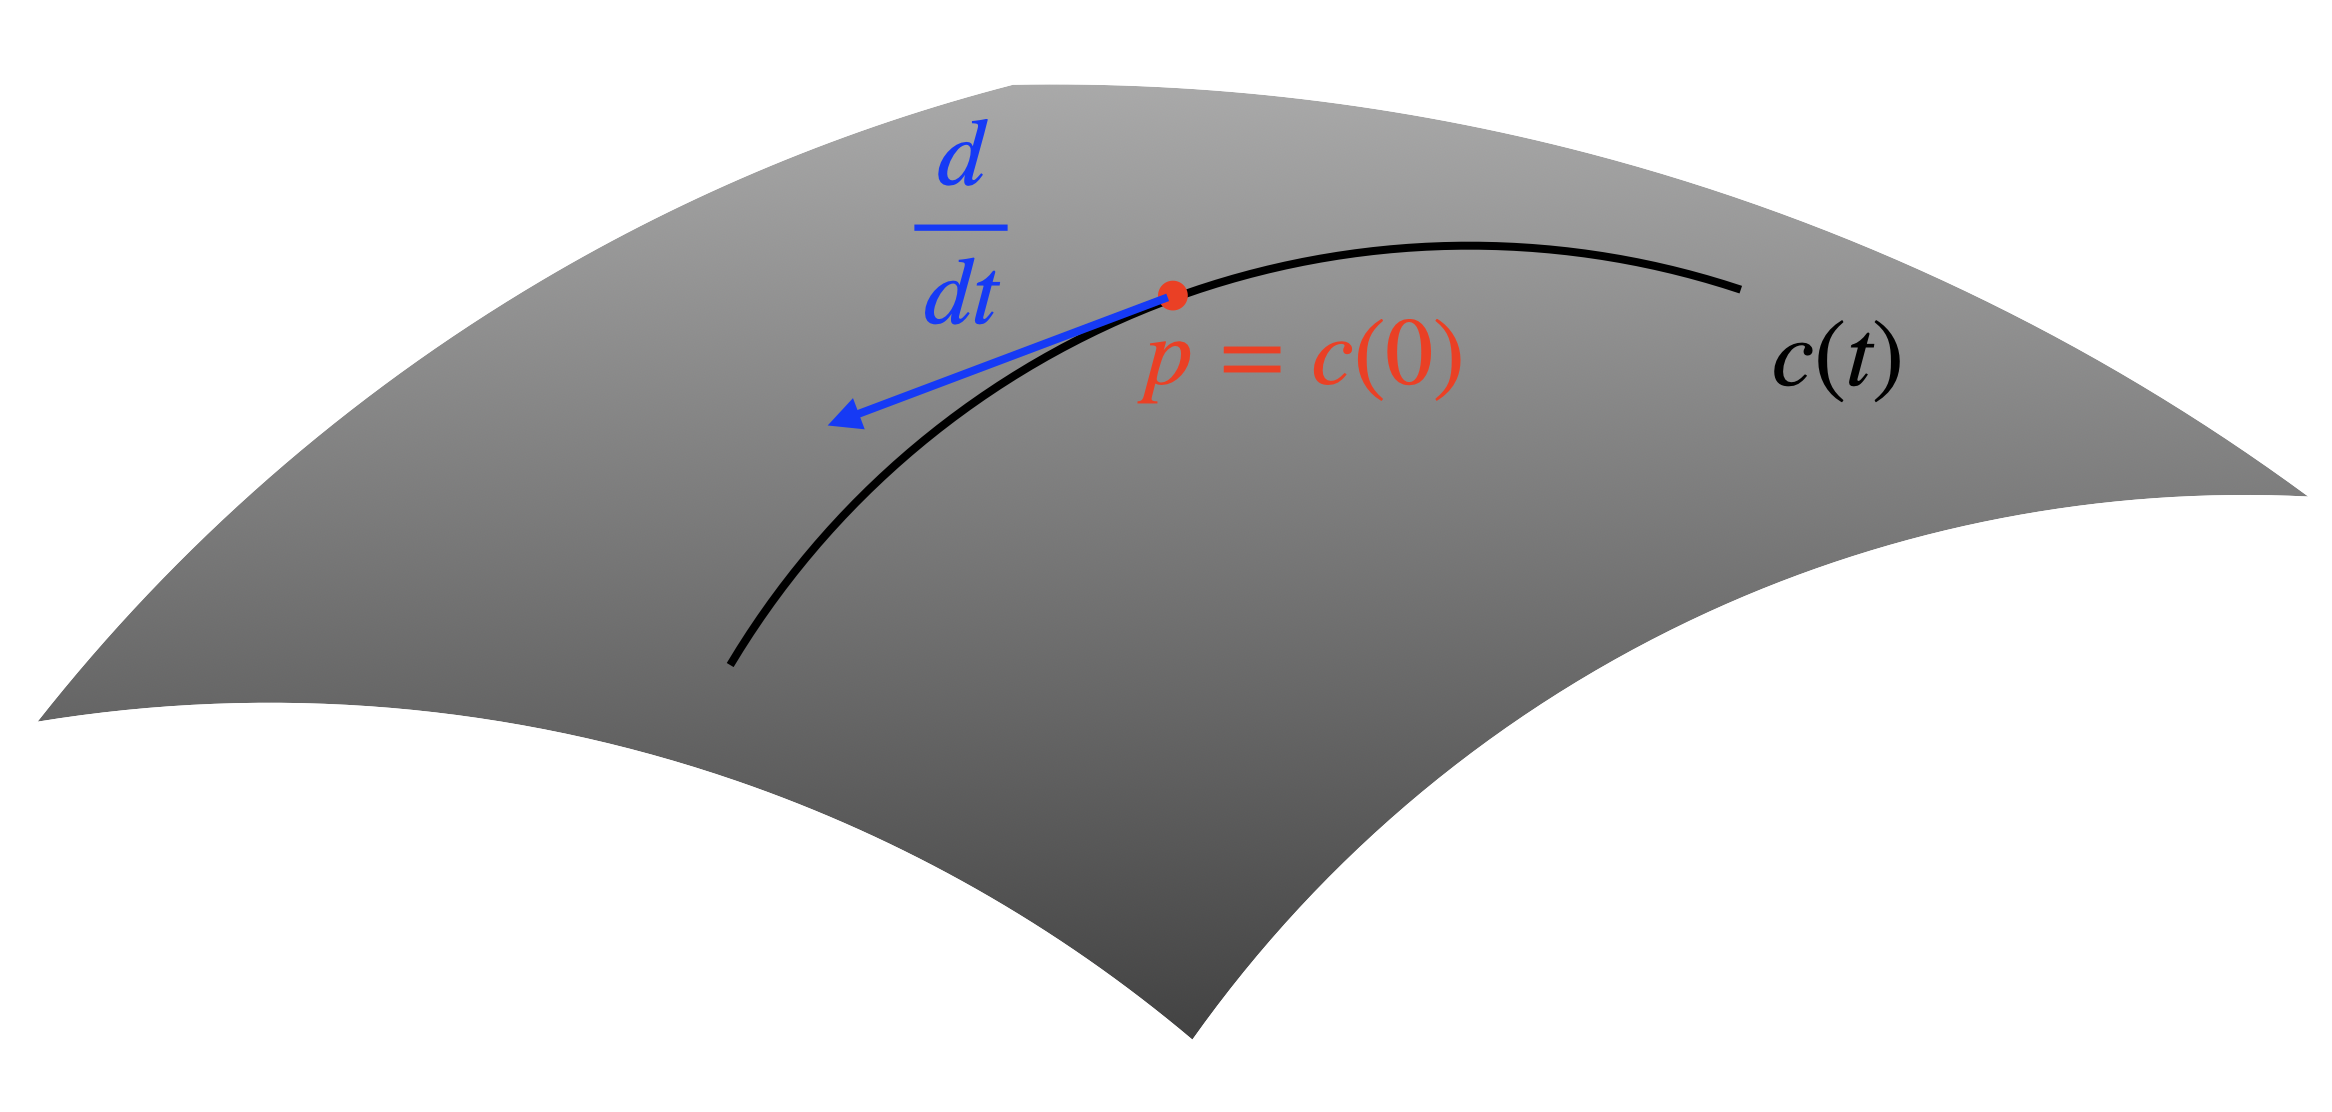
\includegraphics[width=0.5\linewidth]{../images/lecture06/6_01.png}
    \end{figure}

    The rate of change at $t=0$ along $c(t)$ is $\displaystyle{\left.\frac{df(c(t))}{dt}\right|_{t = 0}}$. In terms of the local coordinates $\{x^{\mu}\}$,
    \[ \left.\frac{df(c(t))}{dt}\right|_{t = 0} = \underbrace{\frac{\partial f}{\partial x^{\mu}}}_{(\ast)}\left.\frac{dx^{\mu}(c(t))}{dt}\right|_{t = 0} \]
    We are (again) abusing the notation here. Precisely, $(\ast)$ should be written as $\displaystyle{\frac{\partial(f\circ\varphi^{-1})}{\partial{x}^{\mu}}}$ where $\varphi \,:\, \mca{M} \rightarrow \mbb{R}$ is the coordinate function.
\end{definition}
\newpage

% ===== ===== ===== ===== ===== ===== ===== ===== ===== ===== ===== ===== ===== ===== 

In other words, the derivative is obtained by applying the \tbf{differential operator} $X$ to $f$, defined by
\[ \left.\frac{df(c(t))}{dt}\right|_{t = 0} = \frac{\partial f}{\partial x^{\mu}}\left.\frac{dx^{\mu}(c(t))}{dt}\right|_{t = 0} = \left.\frac{dx^{\mu}(c(t))}{dt}\right|_{t = 0} \cdot \frac{\partial}{\partial x^{\mu}} \cdot f = X^{\mu}\partial_{\mu}f \equiv X[f] \]
where
\[ X = X^{\mu}\partial_{\mu}, \quad X^{\mu} = \left.\frac{dx^{\mu}(c(t))}{dt}\right|_{t = 0} \]
It is $\boxed{X = X^{\mu}\partial_{\mu}}$ which we define as the \tbf{tangent vector} to $\mca{M}$ at $p = c(0)$ along the direction given by the curve $c(t)$!

\seprule

\begin{remark}
    Different curves passing through $p = c(0)$ yields different tangent vectors pointing different directions. Even if the two curves are globally different, but if those has same slope at $p$, they yield same tangent vector.
\end{remark}

\begin{definition}
    Two curves $c_{1}(t)$ and $c_{2}(t)$ are equivalent if
    \begin{align*}
        (i) &\; c_{1}(0) = c_{2}(0) = p \\
        (ii) &\; \left.\frac{dx^{\mu}(c_{1}(t))}{dt}\right|_{t = 0} = \left.\frac{dx^{\mu}(c_{2}(t))}{dt}\right|_{t = 0}
    \end{align*}
    In other words, $c_{1}$ and $c_{2}$ yield the same differential operator. We identify the tangent vector $X$ with the equivalence class of curves.
    \[ [c(t)] = \left\{ \tilde{c}(t) \,|\, \tilde{c}(0) = c(0) \;\text{and}\; \left.\frac{dx^{\mu}(\tilde{c}(t))}{dt}\right|_{t = 0} = \left.\frac{dx^{\mu}(c(t))}{dt}\right|_{t = 0} \right\} \]
\end{definition}

\begin{definition}[Tangent spaces]
    All the equivalence classes of curves at $p \in \mca{M}$, namely all the tangent vectors at $p \in \mca{M}$, form a vector space called the \tbf{tangent space} of $\mca{M}$ at $p$, $T_{p}\mca{M}$.

    \vspace*{1.5em}

    Evidently, $\partial_{\mu}\,(\mu = 1,\,2,\,\cdots,\,m)$ are the \tit{basis vectors} of $T_{p}\mca{M}$.
\end{definition}

\begin{remark}
    \begin{itemize}
        \item[1)] If a vector $V \in T_{p}\mca{M}$ is written as $V = V^{\mu}e_{\mu}$, $V^{\mu}$ are called the components of $V$ with respect to $e_{\mu}$.
        \item[2)] By construction, a vector exists without specifying the coordinates. Coordinate independence property enables us to find the transformation property of the components of the vector. Consider two overlapping charts. For $p \in U_{i} \cap U_{j}$, $x = \varphi_{i}(p)$ and $y = \varphi_{j}(p)$. Two expressions for $X \in T_{p}\mca{M}$ is
        \[ X = X^{\mu}\frac{\partial}{\partial x^{\mu}} = \tilde{X}^{\mu}\frac{\partial}{\partial y^{\mu}} \]
        This gives $\displaystyle{\tilde{X}^{\mu} = X^{\nu}\frac{\partial y^{\mu}}{\partial x^{\nu}}}$
        \item[3)] The basis of $T_{p}\mca{M}$ need not to be $\{e_{\mu}\}$. Linear combinations $\hat{e}_{i} \equiv A_{i}{}^{\mu}e_{\mu}$ where $A = (A_{i}{}^{\mu}) \in \mrm{GL}(m,\mbb{R})$ is also a basis of $T_{p}\mca{M}$: the \tbf{non-coordinate basis}.
    \end{itemize}
\end{remark}
\newpage

% ===== ===== ===== ===== ===== ===== ===== ===== ===== ===== ===== ===== ===== ===== 

\subsection{Cotangent Space}
Since we defined vectors on the manifold, covectors should follow. The dual vector space to $T_{p}\mca{M}$ should take linear maps from $T_{p}\mca{M}$ to $\mbb{R}$ as elements.

\begin{definition}[Cotangent spaces]
    The \tbf{cotangent space} at $p$, $T_{p}^{\ast}\mca{M}$, contains the linear maps $w \,:\, T_{p}\mca{M}\rightarrow\mbb{R}$ (\tbf{dual vector} or \tbf{cotangent vector} or \tbf{one-form}).
    \begin{itemize}
        \item[-] The action of a vector $V$ on $f$ is a \tit{directional derivative}.
        \[ V[f] = V^{\mu}\frac{\partial f}{\partial x^{\mu}} \in \mbb{R} \]
        \item[-] The action of a one-form $\d{f} \in T_{p}^{\ast}\mca{M}$, which is a \tbf{differential} of a smooth function $f \in \mca{F}(\mca{M})$, on $V \in T_{p}\mca{M}$ is defined by
        \[ \left<\d{f}, V\right> \equiv V[f] = V^{\mu}\frac{\partial f}{\partial x^{\mu}} \in \mbb{R} \]
        \item[-] $\d{f}$ is expressed in terms of the coordinate $x = \varphi(p)$ as
        \[ \d{f} = \frac{\partial f}{\partial x^{\mu}} \d{x}^{\mu} \]
        Hence, $\{\d{x}^{\mu}\}$ forms a basis of $T_{p}^{\ast}\mca{M}$ and arbitrary one-form can be expressed as $w = w_{\mu}\d{x}^{\mu}$.
    \end{itemize}
\end{definition}

\begin{definition}[Inner product\footnote{Note that we emphasized that this is not an inner product before. But Nakahara wrote this as an inner product so we follow it.}]
    The \tbf{inner product} $\left<\;,\;\right>\,:\, T_{p}^{\ast}\mca{M} \times T_{p}\mca{M} \rightarrow \mbb{R}$ is defined by
    \[ \left<w, V\right> = w_{\mu}V^{\mu}\left<\d{x}^{\mu},\partial_{\mu}\right> = w_{\mu}V^{\mu} \in \mbb{R} \]
    where $w \in T_{p}^{\ast}\mca{M}$ and $V \in T_{p}\mca{M}$.
\end{definition}

\begin{remark}
    Similar with $X \in T_{p}\mca{M}$, consider $p \in U_{i} \cap U_{j}$ with coordinate functions $x = \varphi_{i}(p)$ and $y = \varphi_{j}(p)$.
    \[ w = w_{\mu}\d{x}^{\mu} = \tilde{w}_{\nu}\d{y}^{\nu} \;\Longrightarrow\; \tilde{w}_{\nu} = w_{\mu}\frac{\partial x^{\mu}}{\partial y^{\nu}} \;\text{since}\; \d{y}^{\nu} = \frac{\partial y^{\nu}}{\partial x^{\mu}} \d{x}^{\mu} \]
\end{remark}

\subsection{Tensors and Tensor Fields}

\begin{definition}
    A \tbf{tensor} of type $(q,r)$ is a multilinear object which maps $q$ elements of $T_{p}^{\ast}\mca{M}$ and $r$ elements of $T_{p}\mca{M}$ to a real number.
    \[ T^{(q,r)} \in \mathfrak{T}_{p}^{(q,r)}(\mca{M}) \;\text{and}\; T^{(q,r)} \,:\, (T_{p}^{\ast}\mca{M})^{\otimes q} \otimes (T_{p}\mca{M})^{\otimes r} \rightarrow \mbb{R} \]
    In component-basis representation,
    \[ T^{(q,r)} = T^{\mu_{1}\cdots \mu_{q}}_{\nu_{1}\cdots\nu_{r}}\frac{\partial}{\partial x^{\mu_{1}}} \otimes \cdots \otimes \frac{\partial}{\partial x^{\mu_{q}}} \otimes \d{x}^{\nu_{1}} \otimes \cdots \otimes \d{x}^{\nu_{r}} \]
\end{definition}
\newpage

% ===== ===== ===== ===== ===== ===== ===== ===== ===== ===== ===== ===== ===== ===== 

\begin{remark}
    For $V_{i} = V_{i}^{\mu}\partial_{\mu}\,(i = 1,\cdots, r)$ and $w_{i} = w_{i\mu}\d{x}^{\mu}\,(i = 1,\cdots,q)$,
    \[ T(w_{1},\cdots,w_{q},V_{1},\cdots,V_{r}) = T^{\mu_{1}\cdots \mu_{q}}_{\nu_{1}\cdots\nu_{r}}w_{1\mu_{1}}\cdots w_{q\mu_{q}}V_{1}^{\nu_{1}}V_{r}^{\nu_{r}} \]
    We use the notation $\left<w, X\right> = w(X)$.
\end{remark}

\begin{definition}
    \hphantom{.}
    \begin{itemize}
        \item[(1)] If a vector is assigned \tit{smoothly} to each point of $\mca{M}$, it is called a \tbf{vector field} over $\mca{M}$. In other words, $V$ is a vector field if $V[f] \in \mca{F}(\mca{M})$ for any $f \in \mca{F}(\mca{M})$. The set of vector fields on $\mca{M}$ is $\mathscr{X}(\mca{M})$.
        \item[(2)] A vector field $X$ restricted at $p \in \mca{M}$ is $X|_{p} \in T_{p}\mca{M}$.
        \item[(3)] A \tbf{tensor field} of type $(q,r)$ is a smooth assignment of an element of $\mathfrak{T}_{p}^{(q,r)}(\mca{M})$ at each $p \in \mca{M}$.
    \end{itemize}
\end{definition}

\subsection{Induced Maps}

\begin{definition}[Pushforward]
    A smooth map $f \,:\, \mca{M} \rightarrow \mca{N}$ naturally induces a \tbf{pushforward} map $f_{\ast} \,:\, T_{p}\mca{M} \rightarrow T_{f(p)}\mca{N}$ as
    \[ (f_{\ast}V)[g] \equiv V[g \circ f] \; \text{\quad} \; V \in T_{p}\mca{M},\, g \in \mca{F}(\mca{N}) \]
\end{definition}

\begin{figure}[htbp]
    \centering
    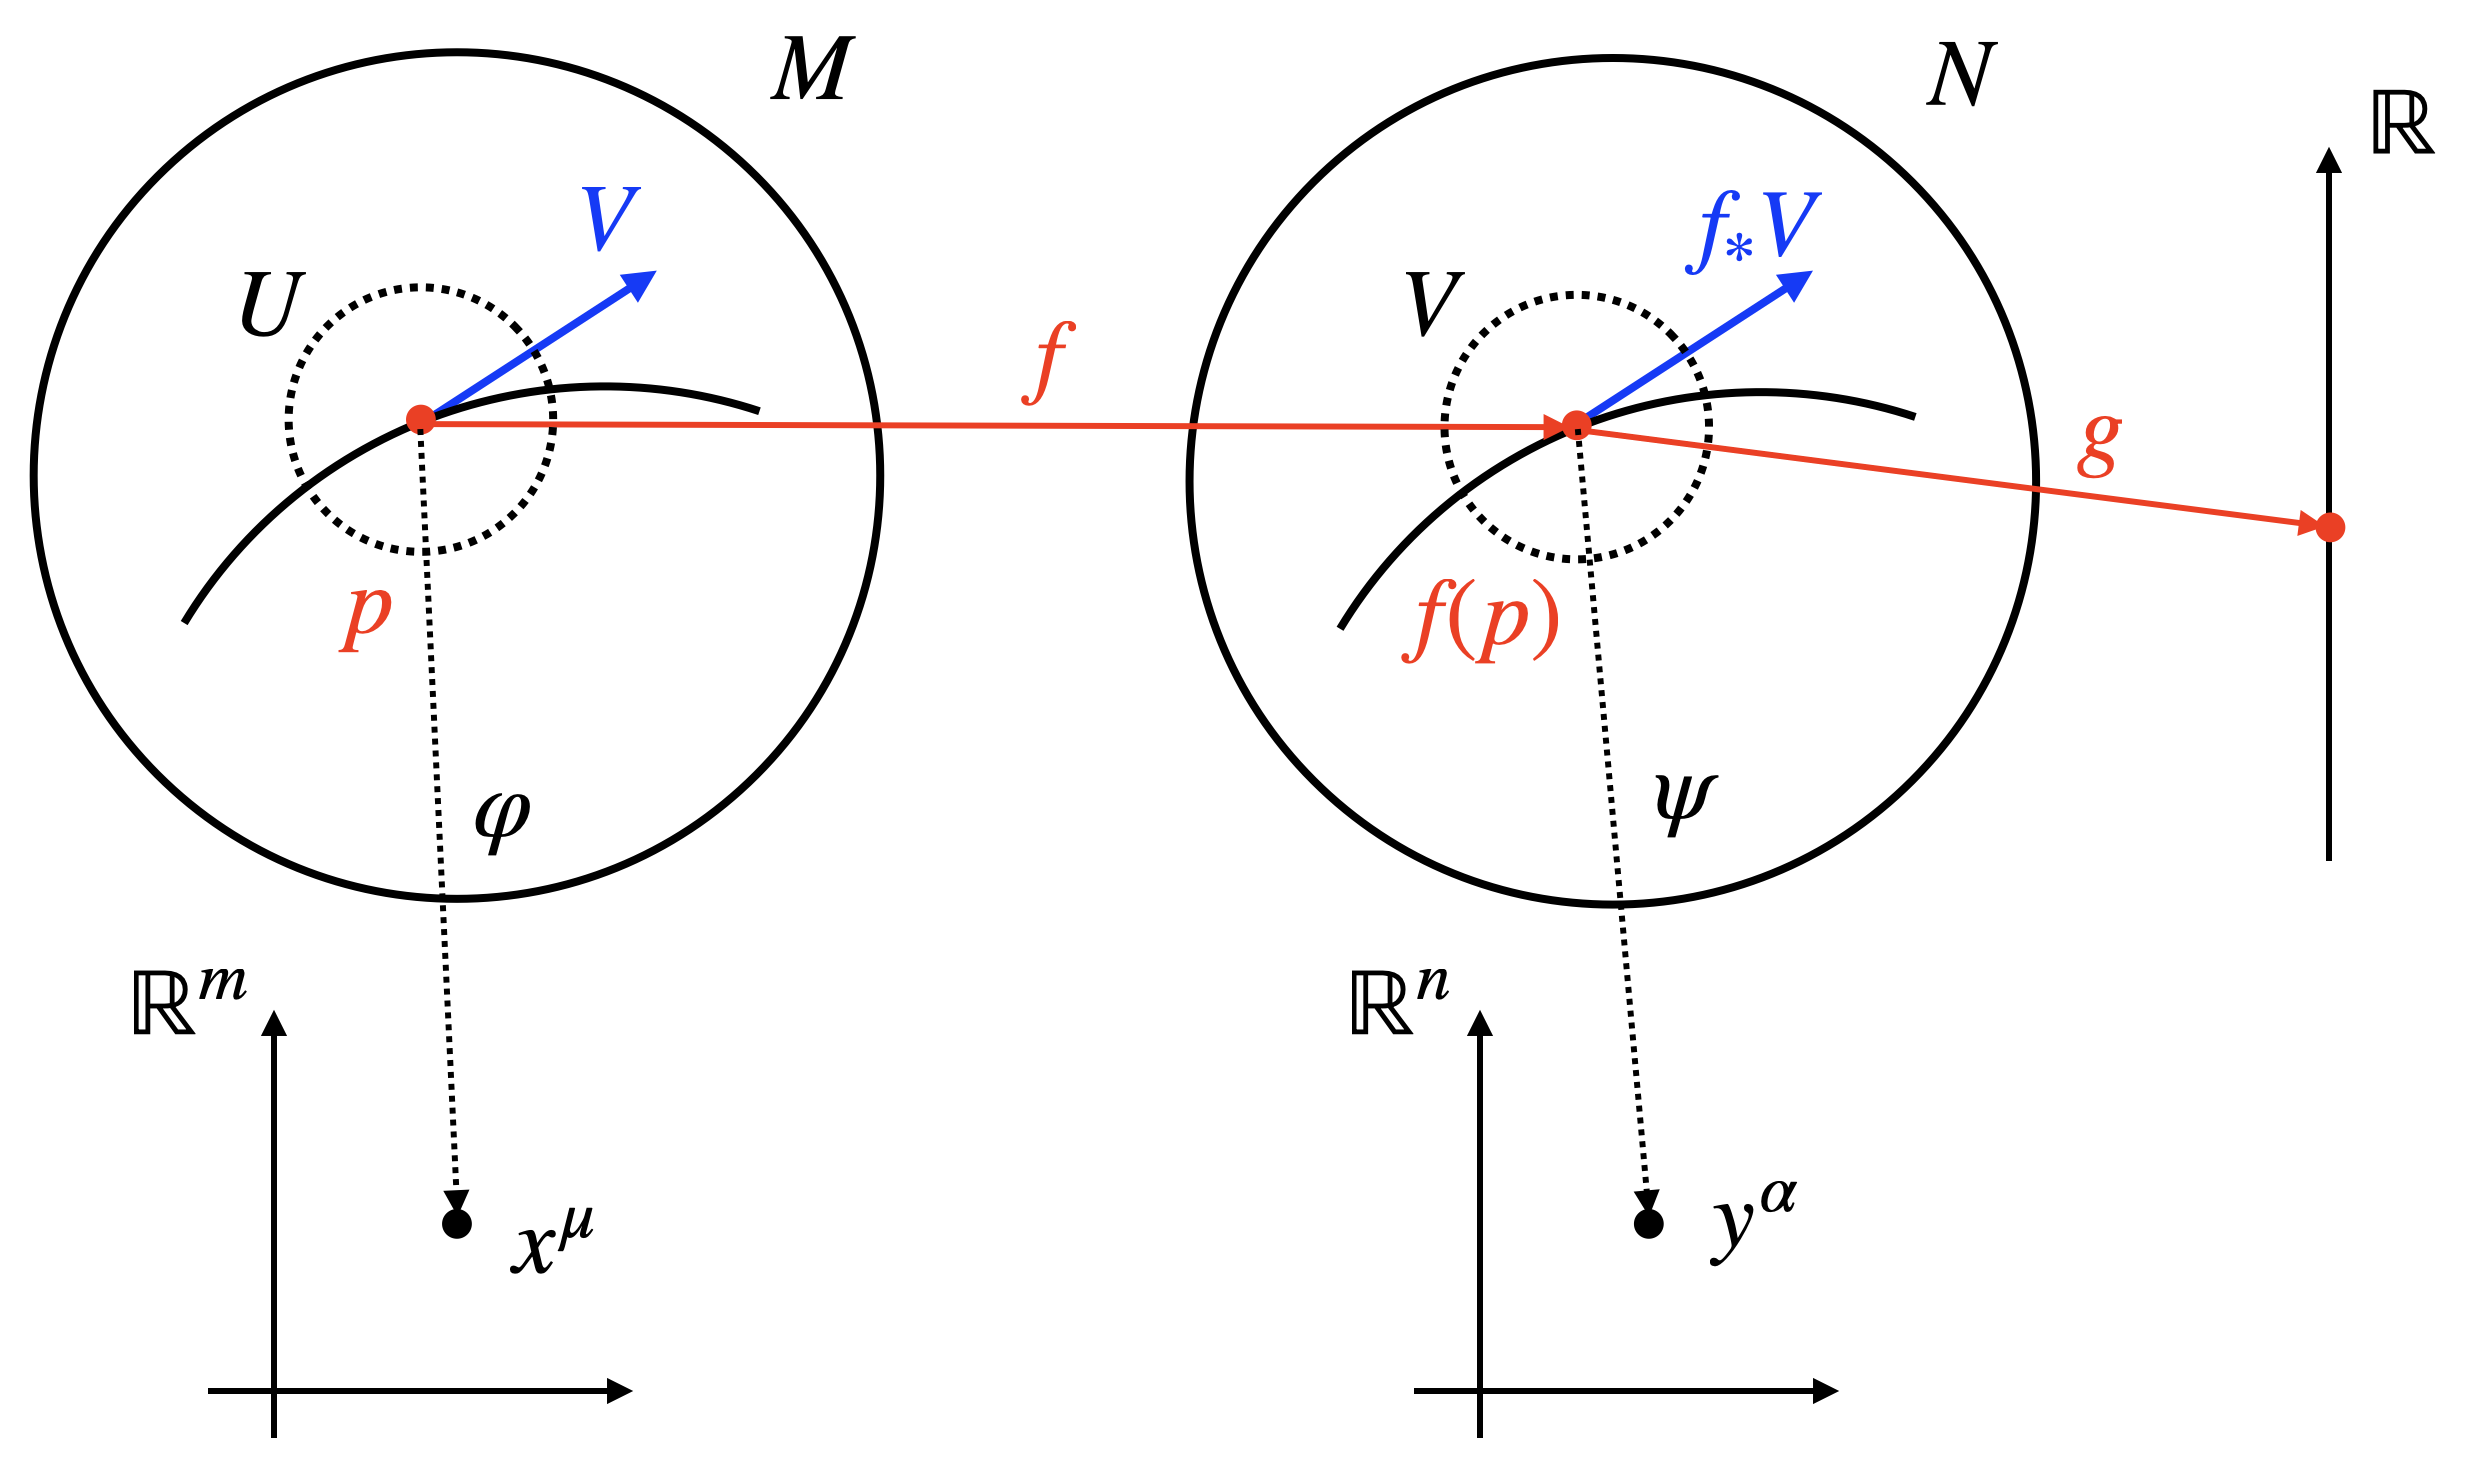
\includegraphics[width=0.8\linewidth]{../images/lecture06/6_02.png}
\end{figure}

In terms of charts $(U, \varphi)$ on $\mca{M}$ and $(V, \psi)$ on $\mca{N}$,
\[ f_{\ast}V[g \circ \psi^{-1}(y)] = V[g\circ f \circ \varphi^{-1}(x)] \]
where $x = \varphi(p)$ and $y = \psi(p)$.
\newpage

% ===== ===== ===== ===== ===== ===== ===== ===== ===== ===== ===== ===== ===== ===== 

\begin{remark}
    Let's compute the components of the pushforward map. Let
    \[ V = V^{\mu}\frac{\partial}{\partial x^{\mu}} \;\text{and}\; f_{\ast}V = W^{\alpha}\frac{\partial}{\partial y^{\alpha}} \]
    Then
    \[ W^{\alpha}\frac{\partial}{\partial y^{\alpha}}[g \circ \psi^{-1}(y)] = V^{\mu}\frac{\partial}{\partial x^{\mu}}[g\circ f\circ \varphi^{-1}(x)] \]
    Take $g = y^{\alpha}$. Then
    \[ W^{\alpha} = V^{\mu}\frac{\partial}{\partial x^{\mu}} y^{\alpha} \]
    where $\partial{y}^{\alpha}/\partial{x}^{\mu}$ is the Jacobian of $f\,:\,\mca{M}\rightarrow\mca{N}$.
\end{remark}
\begin{remark}
    $f_{\ast}$ is naturally extended to tensors of type $(q,0)$.
    \[ f_{\ast} \,:\, \mathfrak{T}^{(q,0)}_{p}(\mca{M}) \rightarrow \mathfrak{T}^{(q,0)}_{f(p)}(\mca{N}) \]
\end{remark}

\begin{exer}
    Let $f\,:\,\mca{M}\rightarrow\mca{N}$ and $g\,:\,\mca{N}\rightarrow\mca{P}$. Show that the pushforward of the composite map $g\circ f\,:\, \mca{M}\rightarrow\mca{P}$ is $(g\circ f)_{\ast} = g_{\ast} \circ f_{\ast}$.
\end{exer}
\begin{proof}
    Consider a map $h \,:\, \mca{P} \rightarrow \mbb{R}$.
    \begin{align*}
        (g \circ f)_{\ast}V[h] &= V[h \circ g \circ f] \\
        &= f_{\ast}V[h \circ g] = g_{\ast}(f_{\ast}V[h]) = (g_{\ast} \circ f_{\ast})V[h]
    \end{align*}
\end{proof}

\seprule

\begin{definition}[Pullback]
    A map $f \,:\, \mca{M} \rightarrow \mca{N}$ also induces a map $f^{\ast} \,:\, T_{f(p)}^{\ast}\mca{N} \rightarrow T_{p}^{\ast}\mca{M}$ (\tbf{pullback map}) as
    \[ \left< f^{\ast}w,\, V\right> = \left< w,\, f_{\ast}V\right> \quad \text{where} \; V \in T_{p}^{\ast}{M},\; w \in T_{f(p)}^{\ast}\mca{N} \]
\end{definition}

\begin{remark}
    Let $w = w_{\alpha}\,\d{y}^{\alpha} \in T_{f(p)}^{\ast}\mca{N}$ and $f^{\ast}w = \xi_{\mu}\,\d{x}^{\mu} \in T_{p}^{\ast}\mca{M}$. Then
    \[ \left<f^{\ast}w,\, V\right> = \left<\xi_{\mu}\,\d{x}^{\mu},\,V^{\nu}\frac{\partial}{\partial x^{\nu}}\right> = \xi_{\mu}V^{\mu} \]
    and
    \[ \left<w,f_{\ast}V\right> = \left<w_{\alpha}\,\d{y}^{\alpha},\,V^{\mu}\frac{\partial{y}^{\nu}}{\partial{x}^{\mu}}\frac{\partial}{\partial{y}^{\nu}}\right> = w_{\alpha}V^{\mu}\frac{\partial{y}^{\alpha}}{\partial{x}^{\mu}} \]
    gives $\displaystyle{\xi_{\mu} = w_{\alpha}\frac{\partial{y}^{\alpha}}{\partial{x}^{\mu}}}$.
\end{remark}

\begin{remark}
    $f^{\ast}$ is naturally extended to tensors of type $(0,r)$.
    \[ f^{\ast} \,:\, \mathfrak{T}^{(0,r)}_{f(p)}(\mca{N}) \rightarrow \mathfrak{T}^{(0,r)}_{p}(\mca{M}) \]
\end{remark}
\newpage

% ===== ===== ===== ===== ===== ===== ===== ===== ===== ===== ===== ===== ===== ===== 

\begin{exer}
    Let $f\,:\,\mca{M}\rightarrow\mca{N}$ and $g\,:\,\mca{N}\rightarrow\mca{P}$. Show that the pullback of the composite map $g\circ f\,:\, \mca{M}\rightarrow\mca{P}$ is $(g\circ f)^{\ast} = f^{\ast} \circ g^{\ast}$.
\end{exer}
\begin{proof}
    \begin{align*}
        \left<(g\circ f)^{\ast}w,\,V\right> &= \left<w,\,(g\circ f)_{\ast}V\right> \\
        &= \left<w,\,(g_{\ast}\circ f_{\ast})V\right> = \left<g^{\ast}w,\,f_{\ast}V\right> = \left<(f^{\ast}\circ g^{\ast})w,\,V\right>
    \end{align*}
\end{proof}

\begin{remark}
    There is no natural extension of the induced map for a tensor of mixed type. The extension is only possible if $f\,:\,\mca{M}\rightarrow\mca{N}$ is a \tit{diffeomorphism}, where the Jacobian of $f^{-1}$ is also defined.
\end{remark}

\begin{definition}
    Let $f\,:\,\mca{M}\rightarrow\mca{N}$ be a smooth map and let $\dim \mca{M} \leq \dim \mca{N}$.
    \begin{itemize}
        \item[(a)] The map $f$ is called an \tbf{immersion} of $\mca{M}$ into $\mca{N}$ if $f_{\ast}\,:\,T_{p}\mca{M}\rightarrow T_{f(p)}\mca{N}$ is an injection\footnote{one-to-one function.}, that is $\mrm{rk}\,f_{\ast} = \dim \mca{M}$.
        \item[(b)] The map $f$ is called an \tbf{embedding} if $f$ is an injection and an immersion. The image $f(\mca{M})$ is called a \tbf{submanifold} of $\mca{N}$.
    \end{itemize}
\end{definition}

\begin{remark}
    If $f$ is an immersion, $f_{\ast}$ maps $T_{p}\mca{M}$ isomorphically to an $m$-dimensional subspace of $T_{f(p)}\mca{N}$.
\end{remark}

\begin{example}
    Consider two maps $f,\,g\,:\,S^{1} \rightarrow \mbb{R}^{2}$.
    
    \begin{figure}[htbp]
        \centering
        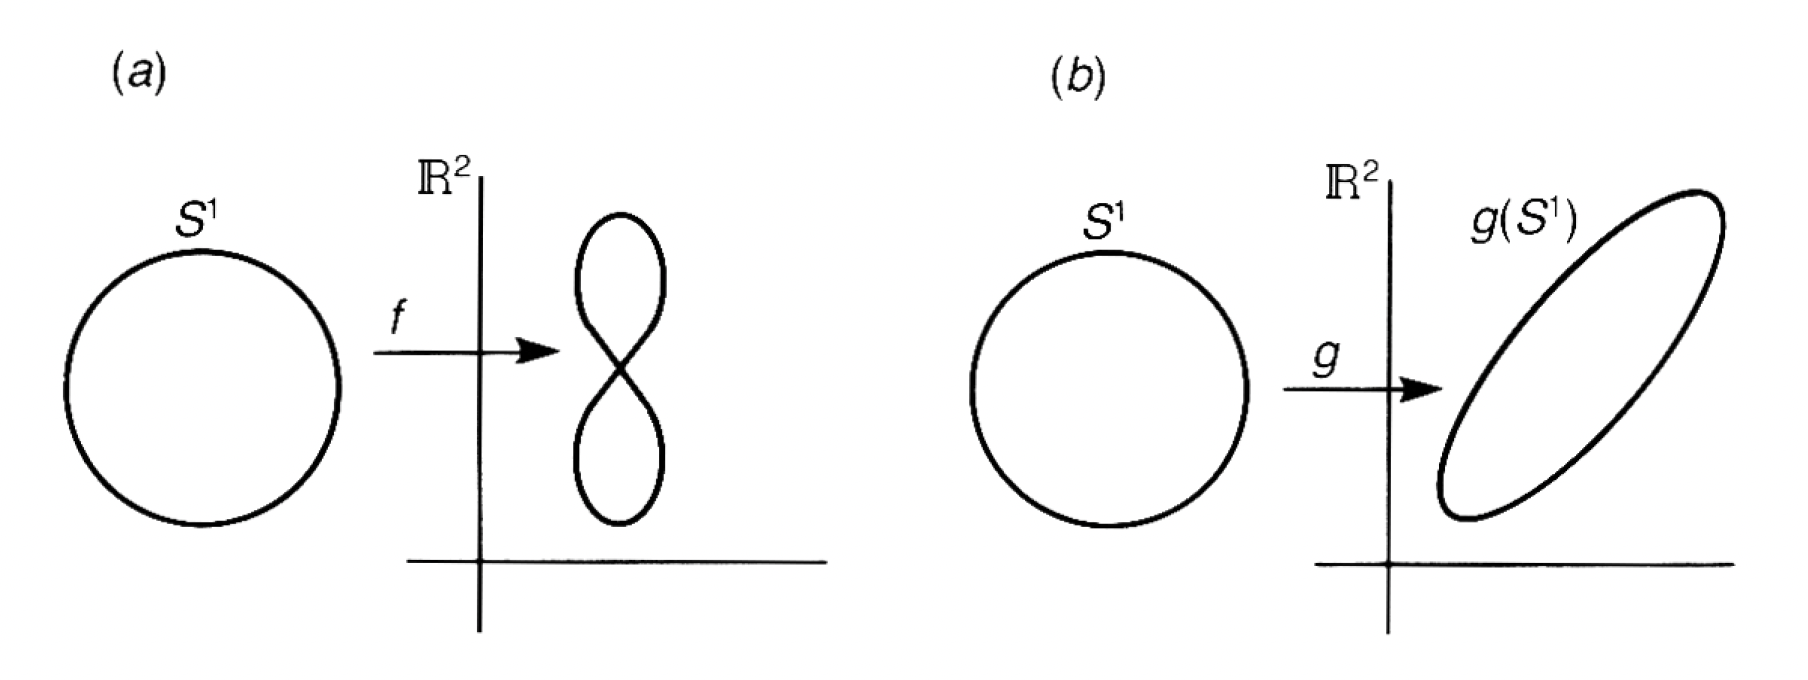
\includegraphics[width=0.8\textwidth]{../images/lecture06/6_03.png}
    \end{figure}

    \begin{itemize}
        \item[-] $f$ is an immersion since a 1D tangent space of $S^{1}$ is mapped by $f_{\ast}$ to a subspace of $T_{f(p)}\mbb{R}^{2}$.
        \item[-] $f(S^{1})$ is not a submanifold of $\mbb{R}^{2}$ since $f$ is not an injection.
        \item[-] $g(S^{1})$ is a submanifold of $\mbb{R}^{2}$, in similar manner.
    \end{itemize}
\end{example}

\end{document}
